%% 
%% Copyright 2019-2021 Elsevier Ltd
%% 
%% This file is part of the 'CAS Bundle'.
%% --------------------------------------
%% 
%% It may be distributed under the conditions of the LaTeX Project Public
%% License, either version 1.2 of this license or (at your option) any
%% later version.  The latest version of this license is in
%%    http://www.latex-project.org/lppl.txt
%% and version 1.2 or later is part of all distributions of LaTeX
%% version 1999/12/01 or later.
%% 
%% The list of all files belonging to the 'CAS Bundle' is
%% given in the file `manifest.txt'.
%% 
%% Template article for cas-dc documentclass for 
%% double column output.

\documentclass[a4paper,fleqn]{cas-dc}

% If the frontmatter runs over more than one page
% use the longmktitle option.

%\documentclass[a4paper,fleqn,longmktitle]{cas-dc}

\usepackage[numbers]{natbib}
%\usepackage[authoryear]{natbib}
% \usepackage[authoryear,longnamesfirst]{natbib}

%%%Author macros
\def\tsc#1{\csdef{#1}{\textsc{\lowercase{#1}}\xspace}}
\tsc{WGM}
\tsc{QE}
%%%

% Uncomment and use as if needed
%\newtheorem{theorem}{Theorem}
%\newtheorem{lemma}[theorem]{Lemma}
%\newdefinition{rmk}{Remark}
%\newproof{pf}{Proof}
%\newproof{pot}{Proof of Theorem \ref{thm}}

\begin{document}
\let\WriteBookmarks\relax
\def\floatpagepagefraction{1}
\def\textpagefraction{.001}

% Short title
% \shorttitle{<short title of the paper for running head>}    
\shorttitle{ATTESS}

% Short author
% \shortauthors{<short author list for running head>}  
\shortauthors{Ketkar Y., Gawade S.}

% Main title of the paper
\title [mode = title]{Detection of Arrhythmia Using Automated Supervised Learning System For COVID-19}

\let\printorcid\relax

% Title footnote mark
% eg: \tnotemark[1]
% \tnotemark[<tnote number>] 

% Title footnote 1.
% eg: \tnotetext[1]{Title footnote text}
% \tnotetext[<tnote number>]{<tnote text>} 

% First author
%
% Options: Use if required
% eg: \author[1,3]{Author Name}[type=editor,
%       style=chinese,
%       auid=000,
%       bioid=1,
%       prefix=Sir,
%       orcid=0000-0000-0000-0000,
%       facebook=<facebook id>,
%       twitter=<twitter id>,
%       linkedin=<linkedin id>,
%       gplus=<gplus id>]

\author[1]{Yashodhan Ketkar}

% Corresponding author indication
% \cormark[<corr mark no>]

% Footnote of the first author
% \fnmark[<footnote mark no>]

% Email id of the first author
\ead{ketkaryapr19me@student.mes.ac.in}

% URL of the first author
% \ead[url]{<URL>}

% Credit authorship
% eg: \credit{Conceptualization of this study, Methodology, Software}
% \credit{<Credit authorship details>}

% Address/affiliation
\affiliation[1]{organization={PCE},
            % addressline={}, 
            city={Panvel},
%          citysep={}, % Uncomment if no comma needed between city and postcode
            postcode={410206}, 
            state={Maharashtra},
            country={India}}

\author[2]{Sushopti Gawade}

% Footnote of the second author
% \fnmark[2]

% Email id of the second author
\ead{sgawade@mes.ac.in}

% URL of the second author
% \ead[url]{}

% Credit authorship
% \credit{}

% Address/affiliation
\affiliation[2]{organization={PCE},
            % addressline={}, 
            city={Panvel},
%          citysep={}, % Uncomment if no comma needed between city and postcode
            postcode={410206}, 
            state={Maharashtra},
            country={India}}

% Corresponding author text
% \cortext[2]{Corresponding author}

% Footnote text
% \fntext[1]{}

% For a title note without a number/mark
%\nonumnote{}

% Here goes the abstract
\begin{abstract}
COVID-19 disease became a global pandemic in the last few years. This disease was highly contagious, and it quickly spread throughout several countries. Its infection can lead to severe implications in its victims, including cardiovascular issues. This complication develops in some people with a history of cardiovascular illness, whereas it emerges in others after COVID-19 infection. Cardiovascular problems are the primary cause of mortality in COVID-19 patients and are used to predict disease prognosis. Identifying arrhythmia from abnormalities in patient ECG signals is one of the few approaches for detecting cardiovascular disorders. This is a laborious and time-consuming procedure that may be automated using a supervised learning technique. Supervised learning is used in the proposed technique to identify abnormalities in ECG frequency waves. The suggested method will then anticipate the presence of arrhythmia in the patient's ECG and notify medical personnel. The suggested technique detects arrhythmia quicker than existing methods and will aid in decreasing the severity of COVID-19 and its complications in infected individuals.
\end{abstract}

% Use if graphical abstract is present
%\begin{graphicalabstract}
%\includegraphics{}
%\end{graphicalabstract}

% Research highlights
% \begin{highlights}
% \item a
% \item a
% \item a
% \end{highlights}

% Keywords
% Each keyword is seperated by \sep
\begin{keywords}
Medical field \sep Machine Learning \sep Supervised ML \sep Prediction
\end{keywords}

\tolerance 9999
\maketitle


% Main text
% \section{Introduction}\label{sec:introduction}
\section{Introduction} \label{sec:introduction}

COVID-19 has been widespread in recent years. It targets the human respiratory system, causing severe respiratory issues. Depending on a person's condition and the prevalence of comorbidities, this disease can be fatal. Cardiovascular comorbidities are frequent in COVID-19 disease. Cardiovascular comorbidities are also problematic to diagnose in the absence of suitable equipment. Checking for arrhythmia in patients is one approach to detection. Arrhythmia is the irregular beating of the heart. Arrhythmia is detected by examining ECG signals. Because COVID-19 has put a strain on the medical personnel, detection takes longer than usual. Increased Internet connectivity has led to the use of machine learning and artificial intelligence (AI) for service in a variety of sectors. This increases research in the field of machine learning and has an impact on machine learning in a variety of domains. One of them is the medical and healthcare businesses. Machine learning is used to detect and categorize viruses and other microorganisms in patients. In medical applications, machine learning algorithms have already been shown to be quite useful.

The machine learning system may be used to scan these ECG signals and detect them. These signs may be detected considerably faster and more efficiently using supervised learning techniques. In such exact classification problems, supervised algorithms have previously been demonstrated to be quicker than unsupervised techniques. Once taught, this algorithm may also be utilized to make future predictions.

There are several supervised algorithms accessible, allowing us to select the best method for our purposes. This phase can be automated in the case of the general population. A few methods may be pre-programmed into the system, and the computer can then train and pick the best model for the supplied dataset. This will free up medical personnel to focus on patient care and problem-solving.

\section{Literature Review} \label{sec:literature_review}
Arrhythmia is one of the most common symptoms in patients with COVID19 \cite{babapoor2020arrhythmia}. Arrhythmia was found in 7\% of all 19 Wuhan COVID cases and 14.8\% of patients with poor outcomes. Data from 17 studies of 5815 patients suggest that up to 9.3\% of confirmed patients detected arrhythmia \cite{mulia2021atrial, liu2020clinical}. Up to 94.4\% of all deceased patients had arrhythmia and 95.8\% of patients with severe infections had arrhythmia \cite{beri2020cardiac, ren2020clinical}. According to the studies \cite{babapoor2020arrhythmia, liu2020clinical, yarmohammadi2021frequency}, only 8\% of patients with arrhythmia had previously had cardiovascular disease, but 56\% of the symptoms of arrhythmia recurred after having COVID19 disease.

In the work \cite{sun2020multi}, the author used an ensemble classifier to detect anomalies in the ECG signal. This approach, which combines multiple classifiers for prediction, has proven effective because the accuracy of the ensemble classifier is significantly higher than that of a single classifier. This approach has also been used by other researchers to improve the prediction accuracy of supervised learning models \cite{huang2020accurate, rajak2020applying, liu2020parallel}. This study also showed high accuracy and validation scores for anomaly detection \cite{huang2020accurate, liu2020parallel}, while one study made accurate predictions without prior information about \cite{rajak2020applying} in the same class. Was shown to be obtained. You can use the default classifier to automatically get an accurate and accurate prediction of the incoming data stream \cite{imbrea2021automated}.

To detect the presence of a patient's epileptic seizure, the authors extracted appropriate features and preprocessed the data by applying supervised and unsupervised machine learning classifiers to the patient. Predictions from test data show that supervised learning models are more effective than unstructured learning models \cite{siddiqui2020review}. The default classifier can be automated for accurate and accurate predictions \cite{imbrea2021automated}. The authors of the \cite{jha2020cardiac} study also showed that a commercially available classifier SVM is very efficient in detecting arrhythmia in the ECG signal.

With the ensemble classifier approach, anomalies can be detected by combining multiple classifiers for prediction. The ensemble classifiers can be more effective and accurate than individual supervised learning models \cite{sun2020multi, liu2020parallel, huang2020accurate}. The author of paper \cite{rajak2020applying} discovered that accurate predictions can be obtained with limited or no prior information about past target values of the same class.

Artificial neural networks are also very effective and accurate in detecting arrhythmia from ECG signals. Neural networks can process raw ECG signals and make predictions \cite{hannun2019cardiologist}. Small neural networks are also very efficient in the recognition process \cite{sannino2018deep}. Neural network predictions are relatively accurate and accurate than known classifiers. Lightweight classifiers such as the LDA classifier showed higher accuracy than SVM classifiers for low energy systems \cite{chen2013design}. The self-adaptive learning algorithm is also efficient for low energy lightweight systems \cite{lei2007afc, owis2002study}. The self-learning algorithm makes the system more dynamic and adapts to incoming signals. This dynamic system takes very little time for identification tasks, but classification tasks are more difficult and very time-consuming.

In the work \cite{natasa2008}, the author uses a two-year dataset collected by Glumo Lake and uses his expertise to train and select models. A mixed approach of data-driven and knowledge-driven modeling is used for the success of the application. As the author of the article \cite{lee2000automatic}, he used loo rate and stop criteria for model selection. The author investigated eight different issues and found that a larger loo rate was more desirable. The authors also suggested that modeling difficulties can only be found by careful numerical calculations.

In the article \cite{malkomes2016bayesian}, a novel kernel is used to get the dataset description. This approach leads to the discovery of invisible models with minimal human interaction. The author of the article \cite{JSSv034i12} created a new model using the glmulti package. These models are unique and flexible. The model is automatically optimized to provide a multi-model interface. This approach allows you to quickly explore a large set of models for selection purposes.
\section{Dataset and Method} \label{sec:dataset_and_method}
\subsection{Method} \label{subsec:method}

\begin{figure}[ht]
    \centering
    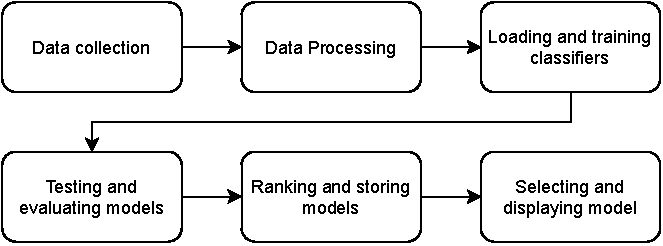
\includegraphics[width=0.7\columnwidth]{media/design/Data_Flow_System.pdf}
    \caption{Training and Selection Process}
    \label{fig:data_flow_in_system}
\end{figure}

The figure \ref{fig:data_flow_in_system}, shows the basic architecture of the automated model training and selection system. The data is collected from the user and processed by the application. This data is stored as training and testing datasets.

\begin{figure}[ht]
    \centering
    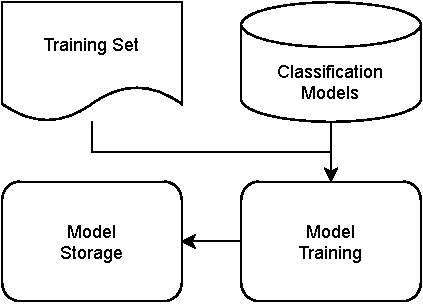
\includegraphics[width=0.7\columnwidth]{media/design/Trainer.pdf}
    \caption{Training Process}
    \label{fig:training_process}
\end{figure}

Figure \ref{fig:training_process}, shows the training process. In this process, the training dataset is loaded into the system. Premade classification model templates are accessed by the system and trained with provided data. These trained models are stored by the system for the next step.

\begin{figure}[ht]
    \centering
    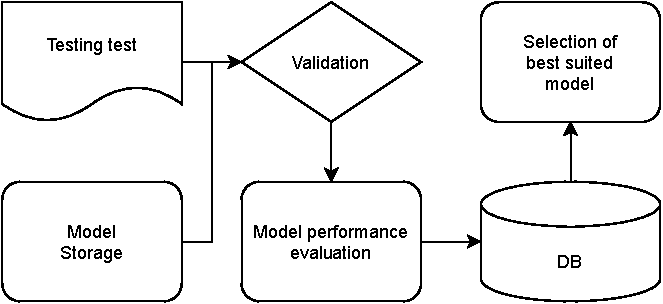
\includegraphics[width=0.7\columnwidth]{media/design/Selector.pdf}
    \caption{Selection Process}
    \label{fig:selection_process}
\end{figure}

The figure \ref{fig:selection_process}, shows the selection process. In this process, the testing dataset is used for the evaluation of the trained models. The trained models are ranked with respect to the performance evaluation. These ranks are used with the help of the tuning parameters to select the best-suited model. This model is stored as the best model for future classification.

\subsection{Dataset}
The ECG readings in this paper are obtained from the MIT-BIH arrhythmia database. This database is used for automated training and evaluation. This dataset was published in 1999 by MIT-BIH as an open-source database; it consists of training and testing datasets. This database is further divided into four equal parts for analysis. Each training set contains 21888 signals, and the testing set contains 5473 signals.
\section{Results And Testing} \label{sec:results_and_testing}
During the automated training and selection process, the SVM classifier is selected as the best-suited model for dataset 1, dataset 2, and dataset 4. Whereas RF classifier is selected as the best-suited model for dataset 3. 

Performance metrics used for evaluation were Accuracy, F1, Precision, Recall, Area under ROC Curve, and Total prediction time. The weightage assigned to these metrics for ranking was 0.65, 0.5, 0.6, 0.6, 0.5, 3 respectively. Where lower value means higher priority.

\subsection{Performance Evaluation} \label{subsec:performance_evaluation}
The models are tested with a testing dataset obtained from MIT-BIH database. Testing dataset consists of 5473 signals. Figure \ref{fig:perfromance_results_dataset_1}, \ref{fig:perfromance_results_dataset_2}, \ref{fig:perfromance_results_dataset_3} and \ref{fig:perfromance_results_dataset_4} shows that model trained with automated system produced satisfactory results. Few models like KNN, RF, and SVM performed better than other models (DT) at the cost of higher prediction time. Whereas MLP models produced good overall results with lower prediction time.

% Best model Performance tabular
\begin{table}[hbt]
\caption{Performance of models trained on dataset 1} \label{tab:performance_of_models_trained_on_dataset_1}
\begin{tabular*}{\tblwidth}{@{}LLLLLL@{}}
    \toprule
    Metric & KNN & DT & MLP & RF & \textbf{SVM} \\
    \midrule
    Accuracy & 96.72 & 94.46 & 96.89 & 97.33 & \textbf{97.40} \\
    F1 & 89.71 & 83.43 & 90.05 & 91.30 & \textbf{91.69} \\
    Precision & 92.53 & 81.86 & 94.71 & 97.95 & \textbf{96.43} \\
    Recall & 87.06 & 85.06 & 85.84 & 85.50 & \textbf{87.40} \\
    ROC & 92.84 & 90.68 & 92.45 & 92.57 & \textbf{93.38} \\
    Time(s) & 0.457 & 0.001 & 0.002 & 0.015 & \textbf{0.297} \\
    \bottomrule
\end{tabular*}
\end{table}

\begin{table}[hbt]
\caption{Performance of models trained on dataset 2} \label{tab:performance_of_models_trained_on_dataset_2}
\begin{tabular*}{\tblwidth}{@{}LLLLLL@{}}
    \toprule
    Metric & KNN & DT & MLP & RF & \textbf{SVM} \\
    \midrule
    Accuracy & 96.83 & 95.04 & 96.69 & 97.09 & \textbf{97.46} \\
    F1 & 90.28 & 85.50 & 89.73 & 90.75 & \textbf{92.15} \\
    Precision & 94.25 & 84.90 & 94.73 & 98.60 & \textbf{96.79} \\
    Recall & 86.63 & 86.09 & 85.23 & 84.05 & \textbf{87.93} \\
    ROC & 92.77 & 91.48 & 92.13 & 91.90 & \textbf{93.66} \\
    Time(s) & 0.435 & 0.001 & 0.003 & 0.014 & \textbf{0.295} \\
    \bottomrule
\end{tabular*}
\end{table}

\begin{table}[hbt]
\caption{Performance of models trained on dataset 3} \label{tab:performance_of_models_trained_on_dataset_3}
\begin{tabular*}{\tblwidth}{@{}LLLLLL@{}}
    \toprule
    Metric & KNN & DT & MLP & \textbf{RF} & SVM \\
    \midrule
    Accuracy & 97.07 & 94.64 & 96.41 & \textbf{97.22} & 97.44 \\
    F1 & 90.93 & 84.30 & 89.34 & \textbf{91.21} & 92.00 \\
    Precision & 95.82 & 83.81 & 90.13 & \textbf{98.37} & 97.81 \\
    Recall & 86.53 & 84.80 & 88.57 & \textbf{85.02} & 86.85 \\
    ROC & 92.87 & 90.73 & 93.29 & \textbf{92.36} & 93.22 \\
    Time(s) & 0.404 & 0.001 & 0.002 & \textbf{0.017} & 0.293 \\
    \bottomrule
\end{tabular*}
\end{table}

\begin{table}[hbt]
\caption{Performance of models trained on dataset 4} \label{tab:performance_of_models_trained_on_dataset_4}
\begin{tabular*}{\tblwidth}{@{}LLLLLL@{}}
    \toprule
    Metric & KNN & DT & MLP & RF & \textbf{SVM} \\
    \midrule
    Accuracy & 96.84 & 94.99 & 95.34 & 96.88 & \textbf{97.15} \\
    F1 & 90.52 & 85.73 & 85.01 & 90.37 & \textbf{91.39} \\
    Precision & 95.71 & 85.91 & 97.83 & 98.65 & \textbf{97.41} \\
    Recall & 85.86 & 85.55 & 75.15 & 83.37 & \textbf{86.07} \\
    ROC & 92.52 & 91.28 & 87.40 & 91.56 & \textbf{92.79} \\
    Time(s) & 0.452 & 0.001 & 0.002 & 0.014 & \textbf{0.294} \\
    \bottomrule
\end{tabular*}
\end{table}

% Best model Performance chart
\begin{figure}[btp]
    \centering
    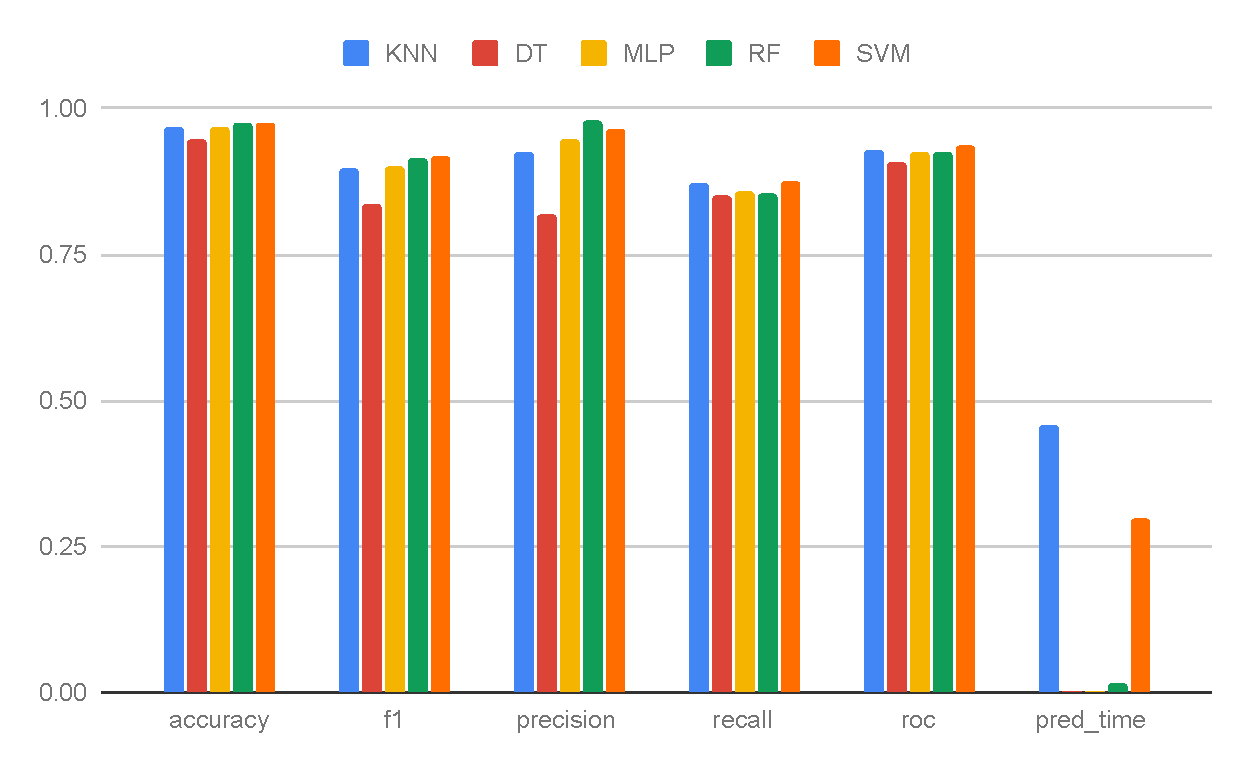
\includegraphics[width=0.9\columnwidth]{media/results/perf_ds_1.pdf}
    \caption{Performance Results Dataset 1} \label{fig:perfromance_results_dataset_1}
\end{figure}

\begin{figure}[btp]
    \centering
    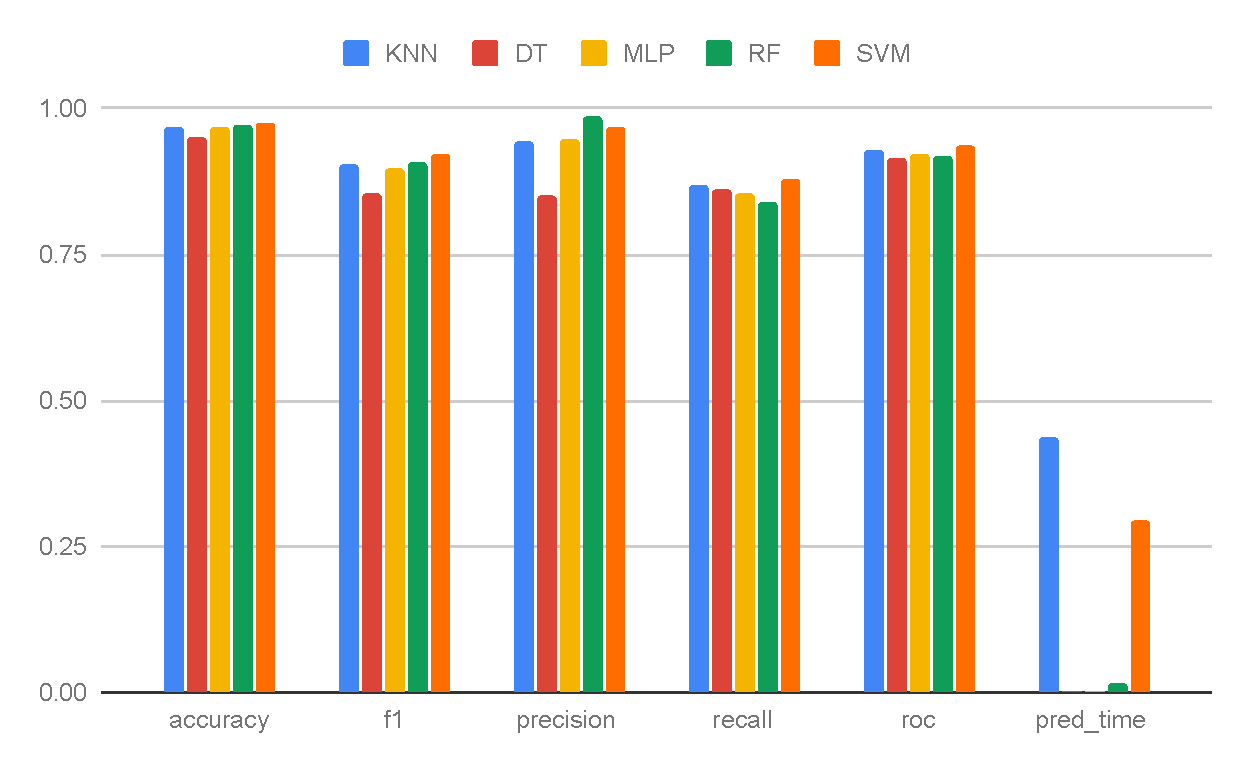
\includegraphics[width=0.9\columnwidth]{media/results/perf_ds_2.pdf}
    \caption{Performance Results Dataset 2} \label{fig:perfromance_results_dataset_2}
\end{figure}

\begin{figure}[btp]
    \centering
    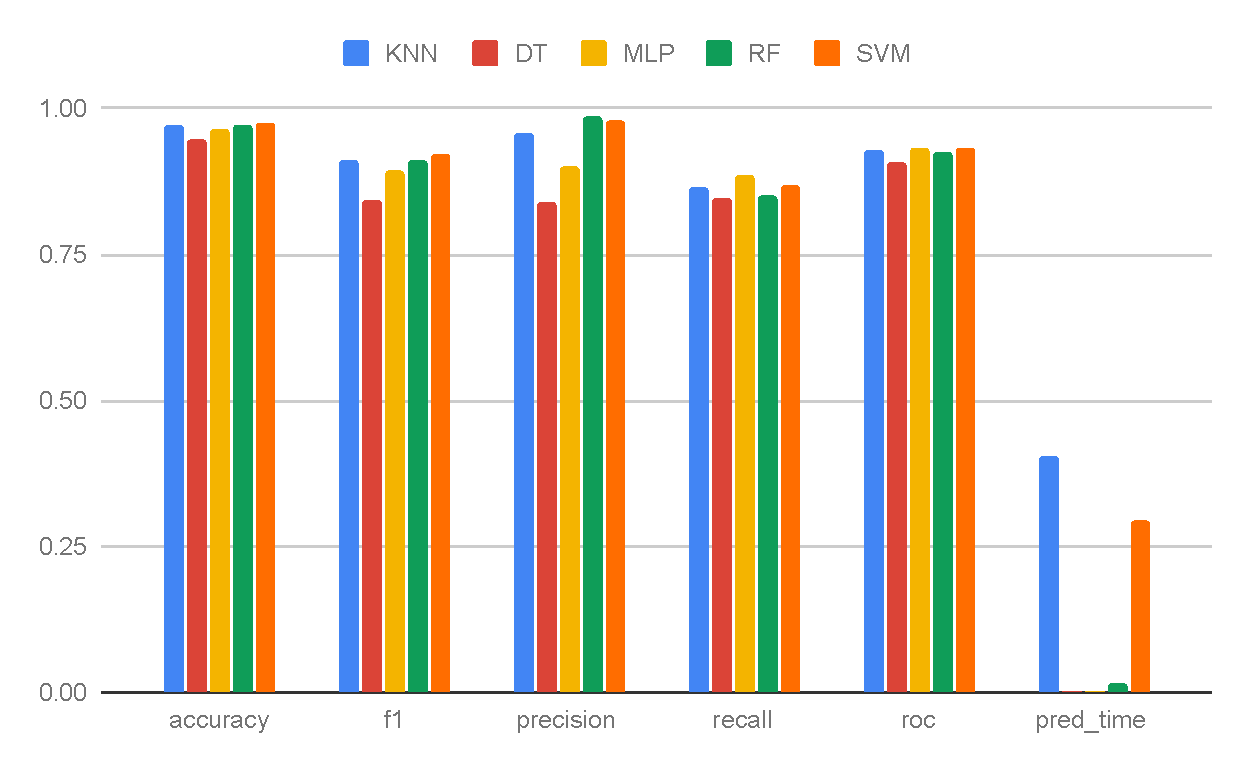
\includegraphics[width=0.9\columnwidth]{media/results/perf_ds_3.pdf}
    \caption{Performance Results Dataset 3} \label{fig:perfromance_results_dataset_3}
\end{figure}

\begin{figure}[btp]
    \centering
    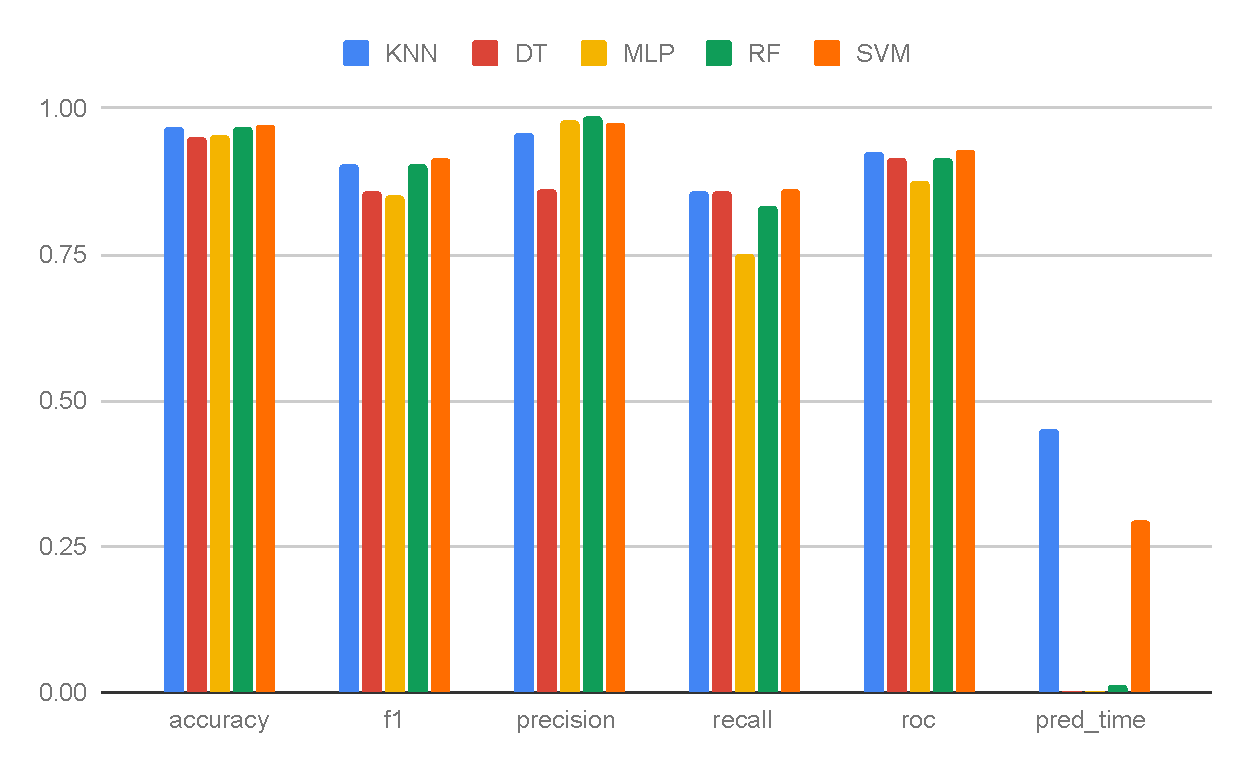
\includegraphics[width=0.9\columnwidth]{media/results/perf_ds_4.pdf}
    \caption{Performance Results Dataset 4} \label{fig:perfromance_results_dataset_4}
\end{figure}

\subsection{Performance Error Calculation}
For error calculation, best models are tested against training datasets of other models. Figure \ref{fig:perfromance_delta_knn}-\ref{fig:perfromance_delta_svm} shows the average error introduced when models are tested against training datasets of other models. This chart shows that KNN, MLP, and SVM models introduced minimum errors, whereas DT and RF models introduced large amounts of error. Figure \ref{fig:perfromance_delta_svm} also shows that SVM model produced similar error across all datasets. This smaller difference in error suggests that the SVM classifier can be used for classification tasks of similar nature.

% Decision Tree Cross-Performance
\begin{table}[hbt]
\caption{Performance of Decision Tree model trained on dataset 1}\label{tab:performance_of_decision_tree_model_trained_on_dataset_1}
\begin{tabular*}{\tblwidth}{@{}LLLLL@{}}
\toprule
    Metric & Dataset 1 & Dataset 2 & Dataset 3 & Dataset 4 \\
\midrule
    Accuracy & 0.98 & 0.94 & 0.94 & 0.94 \\
    F1 & 0.96 & 0.85 & 0.85 & 0.84 \\
    Precision & 0.95 & 0.83 & 0.84 & 0.83 \\
    Recall & 0.96 & 0.86 & 0.85 & 0.85 \\
    ROC & 0.97 & 0.91 & 0.91 & 0.90 \\
\bottomrule
\end{tabular*}
\end{table}

\begin{table}[hbt]
\caption{Performance of Decision Tree model trained on dataset 2}\label{tab:performance_of_decision_tree_model_trained_on_dataset_2}
\begin{tabular*}{\tblwidth}{@{}LLLLL@{}}
\toprule
    Metric & Dataset 1 & Dataset 2 & Dataset 3 & Dataset 4 \\
\midrule
    Accuracy & 0.94 & 0.98 & 0.94 & 0.94 \\
    F1 & 0.84 & 0.96 & 0.84 & 0.85 \\
    Precision & 0.85 & 0.96 & 0.85 & 0.85 \\
    Recall & 0.82 & 0.96 & 0.84 & 0.84 \\
    ROC & 0.89 & 0.97 & 0.90 & 0.90 \\
\bottomrule
\end{tabular*}
\end{table}

\begin{table}[hbt]
\caption{Performance of Decision Tree model trained on dataset 3}\label{tab:performance_of_decision_tree_model_trained_on_dataset_3}
\begin{tabular*}{\tblwidth}{@{}LLLLL@{}}
\toprule
    Metric & Dataset 1 & Dataset 2 & Dataset 3 & Dataset 4 \\
\midrule
    Accuracy & 0.94 & 0.94 & 0.98 & 0.94 \\
    F1 & 0.84 & 0.84 & 0.96 & 0.83 \\
    Precision & 0.84 & 0.83 & 0.95 & 0.83 \\
    Recall & 0.84 & 0.85 & 0.96 & 0.84 \\
    ROC & 0.90 & 0.90 & 0.97 & 0.90 \\
\bottomrule
\end{tabular*}
\end{table}

\begin{table}[hbt]
\caption{Performance of Decision Tree model trained on dataset 4}\label{tab:performance_of_decision_tree_model_trained_on_dataset_4}
\begin{tabular*}{\tblwidth}{@{}LLLLL@{}}
\toprule
    Metric & Dataset 1 & Dataset 2 & Dataset 3 & Dataset 4 \\
\midrule
    Accuracy & 0.94 & 0.94 & 0.95 & 0.98 \\
    F1 & 0.85 & 0.85 & 0.85 & 0.96 \\
    Precision & 0.85 & 0.85 & 0.85 & 0.96 \\
    Recall & 0.85 & 0.84 & 0.85 & 0.96 \\
    ROC & 0.91 & 0.90 & 0.91 & 0.97 \\
\bottomrule
\end{tabular*}
\end{table}

% KNN Cross-Performance
\begin{table}[hbt]
\caption{Performance of KNN model trained on dataset 1}\label{tab:performance_of_knn_model_trained_on_dataset_1}
\begin{tabular*}{\tblwidth}{@{}LLLLL@{}}
\toprule
    Metric & Dataset 1 & Dataset 2 & Dataset 3 & Dataset 4 \\
\midrule
    Accuracy & 0.97 & 0.97 & 0.97 & 0.96 \\
    F1 & 0.93 & 0.91 & 0.90 & 0.90 \\
    Precision & 0.96 & 0.95 & 0.94 & 0.94 \\
    Recall & 0.90 & 0.87 & 0.87 & 0.87 \\
    ROC & 0.94 & 0.93 & 0.93 & 0.93 \\
\bottomrule
\end{tabular*}
\end{table}

\begin{table}[hbt]
\caption{Performance of KNN model trained on dataset 2}\label{tab:performance_of_knn_model_trained_on_dataset_2}
\begin{tabular*}{\tblwidth}{@{}LLLLL@{}}
\toprule
    Metric & Dataset 1 & Dataset 2 & Dataset 3 & Dataset 4 \\
\midrule
    Accuracy & 0.96 & 0.97 & 0.96 & 0.96 \\
    F1 & 0.90 & 0.93 & 0.90 & 0.89 \\
    Precision & 0.94 & 0.96 & 0.94 & 0.94 \\
    Recall & 0.86 & 0.90 & 0.86 & 0.85 \\
    ROC & 0.92 & 0.94 & 0.92 & 0.92 \\
\bottomrule
\end{tabular*}
\end{table}

\begin{table}[hbt]
\caption{Performance of KNN model trained on dataset 3}\label{tab:performance_of_knn_model_trained_on_dataset_3}
\begin{tabular*}{\tblwidth}{@{}LLLLL@{}}
\toprule
    Metric & Dataset 1 & Dataset 2 & Dataset 3 & Dataset 4 \\
\midrule
    Accuracy & 0.96 & 0.96 & 0.97 & 0.96 \\
    F1 & 0.90 & 0.90 & 0.93 & 0.90 \\
    Precision & 0.95 & 0.95 & 0.96 & 0.94 \\
    Recall & 0.86 & 0.86 & 0.89 & 0.86 \\
    ROC & 0.92 & 0.92 & 0.94 & 0.92 \\
\bottomrule
\end{tabular*}
\end{table}

\begin{table}[hbt]
\caption{Performance of KNN model trained on dataset 4}\label{tab:performance_of_knn_model_trained_on_dataset_4}
\begin{tabular*}{\tblwidth}{@{}LLLLL@{}}
\toprule
    Metric & Dataset 1 & Dataset 2 & Dataset 3 & Dataset 4 \\
\midrule
    Accuracy & 0.96 & 0.96 & 0.96 & 0.97 \\
    F1 & 0.90 & 0.90 & 0.90 & 0.92 \\
    Precision & 0.94 & 0.95 & 0.94 & 0.96 \\
    Recall & 0.86 & 0.86 & 0.87 & 0.89 \\
    ROC & 0.92 & 0.92 & 0.93 & 0.94 \\
\bottomrule
\end{tabular*}
\end{table}

% MLP Cross-Performance
\begin{table}[hbt]
\caption{Performance of MLP model trained on dataset 1}\label{tab:performance_of_mlp_model_trained_on_dataset_1}
\begin{tabular*}{\tblwidth}{@{}LLLLL@{}}
\toprule
    Metric & Dataset 1 & Dataset 2 & Dataset 3 & Dataset 4 \\
\midrule
    Accuracy & 0.97 & 0.96 & 0.96 & 0.96 \\
    F1 & 0.92 & 0.89 & 0.89 & 0.89 \\
    Precision & 0.97 & 0.95 & 0.94 & 0.95 \\
    Recall & 0.88 & 0.85 & 0.85 & 0.85 \\
    ROC & 0.93 & 0.92 & 0.92 & 0.92 \\
\bottomrule
\end{tabular*}
\end{table}

\begin{table}[hbt]
\caption{Performance of MLP model trained on dataset 2}\label{tab:performance_of_mlp_model_trained_on_dataset_2}
\begin{tabular*}{\tblwidth}{@{}LLLLL@{}}
\toprule
    Metric & Dataset 1 & Dataset 2 & Dataset 3 & Dataset 4 \\
\midrule
    Accuracy & 0.96 & 0.97 & 0.96 & 0.96 \\
    F1 & 0.90 & 0.91 & 0.90 & 0.90 \\
    Precision & 0.95 & 0.97 & 0.94 & 0.95 \\
    Recall & 0.85 & 0.87 & 0.85 & 0.85 \\
    ROC & 0.92 & 0.93 & 0.92 & 0.92 \\
\bottomrule
\end{tabular*}
\end{table}

\begin{table}[hbt]
\caption{Performance of MLP model trained on dataset 3}\label{tab:performance_of_mlp_model_trained_on_dataset_3}
\begin{tabular*}{\tblwidth}{@{}LLLLL@{}}
\toprule
    Metric & Dataset 1 & Dataset 2 & Dataset 3 & Dataset 4 \\
\midrule
    Accuracy & 0.96 & 0.96 & 0.96 & 0.96 \\
    F1 & 0.89 & 0.89 & 0.90 & 0.88 \\
    Precision & 0.89 & 0.89 & 0.90 & 0.89 \\
    Recall & 0.88 & 0.88 & 0.91 & 0.88 \\
    ROC & 0.93 & 0.93 & 0.94 & 0.93 \\
\bottomrule
\end{tabular*}
\end{table}

\begin{table}[hbt]
\caption{Performance of MLP model trained on dataset 4}\label{tab:performance_of_mlp_model_trained_on_dataset_4}
\begin{tabular*}{\tblwidth}{@{}LLLLL@{}}
\toprule
    Metric & Dataset 1 & Dataset 2 & Dataset 3 & Dataset 4 \\
\midrule
    Accuracy & 0.95 & 0.95 & 0.95 & 0.95 \\
    F1 & 0.85 & 0.85 & 0.85 & 0.86 \\
    Precision & 0.97 & 0.97 & 0.97 & 0.98 \\
    Recall & 0.75 & 0.75 & 0.75 & 0.76 \\
    ROC & 0.87 & 0.87 & 0.87 & 0.88 \\
\bottomrule
\end{tabular*}
\end{table}

% RF Cross-Performance
\begin{table}[hbt]
\caption{Performance of RF model trained on dataset 1}\label{tab:performance_of_rf_model_trained_on_dataset_1}
\begin{tabular*}{\tblwidth}{@{}LLLLL@{}}
\toprule
    Metric & Dataset 1 & Dataset 2 & Dataset 3 & Dataset 4 \\
\midrule
    Accuracy & 0.99 & 0.97 & 0.97 & 0.97 \\
    F1 & 0.98 & 0.91 & 0.91 & 0.91 \\
    Precision & 0.99 & 0.98 & 0.97 & 0.98 \\
    Recall & 0.96 & 0.85 & 0.85 & 0.85 \\
    ROC & 0.98 & 0.92 & 0.92 & 0.92 \\
\bottomrule
\end{tabular*}
\end{table}

\begin{table}[hbt]
\caption{Performance of RF model trained on dataset 2}\label{tab:performance_of_rf_model_trained_on_dataset_2}
\begin{tabular*}{\tblwidth}{@{}LLLLL@{}}
\toprule
    Metric & Dataset 1 & Dataset 2 & Dataset 3 & Dataset 4 \\
\midrule
    Accuracy & 0.96 & 0.99 & 0.97 & 0.97 \\
    F1 & 0.90 & 0.97 & 0.91 & 0.90 \\
    Precision & 0.98 & 0.99 & 0.97 & 0.98 \\
    Recall & 0.83 & 0.96 & 0.85 & 0.84 \\
    ROC & 0.91 & 0.98 & 0.92 & 0.91 \\
\bottomrule
\end{tabular*}
\end{table}

\begin{table}[hbt]
\caption{Performance of RF model trained on dataset 3}\label{tab:performance_of_rf_model_trained_on_dataset_3}
\begin{tabular*}{\tblwidth}{@{}LLLLL@{}}
\toprule
    Metric & Dataset 1 & Dataset 2 & Dataset 3 & Dataset 4 \\
\midrule
    Accuracy & 0.96 & 0.97 & 0.99 & 0.97 \\
    F1 & 0.90 & 0.90 & 0.97 & 0.90 \\
    Precision & 0.98 & 0.98 & 0.99 & 0.98 \\
    Recall & 0.83 & 0.84 & 0.96 & 0.83 \\
    ROC & 0.91 & 0.91 & 0.98 & 0.91 \\
\bottomrule
\end{tabular*}
\end{table}

\begin{table}[hbt]
\caption{Performance of RF model trained on dataset 4}\label{tab:performance_of_rf_model_trained_on_dataset_4}
\begin{tabular*}{\tblwidth}{@{}LLLLL@{}}
\toprule
    Metric & Dataset 1 & Dataset 2 & Dataset 3 & Dataset 4 \\
\midrule
    Accuracy & 0.96 & 0.97 & 0.97 & 0.99 \\
    F1 & 0.90 & 0.91 & 0.90 & 0.97 \\
    Precision & 0.98 & 0.98 & 0.97 & 0.99 \\
    Recall & 0.84 & 0.84 & 0.85 & 0.95 \\
    ROC & 0.91 & 0.92 & 0.92 & 0.97 \\
\bottomrule
\end{tabular*}
\end{table}

% SVM Cross-Performance
\begin{table}[hbt]
\caption{Performance of SVM model trained on dataset 1}\label{tab:performance_of_svm_model_trained_on_dataset_1}
\begin{tabular*}{\tblwidth}{@{}LLLLL@{}}
\toprule
    Metric & Dataset 1 & Dataset 2 & Dataset 3 & Dataset 4 \\
\midrule
    Accuracy & 0.97 & 0.97 & 0.97 & 0.97 \\
    F1 & 0.93 & 0.92 & 0.91 & 0.91 \\
    Precision & 0.98 & 0.97 & 0.96 & 0.96 \\
    Recall & 0.89 & 0.87 & 0.87 & 0.87 \\
    ROC & 0.94 & 0.93 & 0.93 & 0.93 \\
\bottomrule
\end{tabular*}
\end{table}

\begin{table}[hbt]
\caption{Performance of SVM model trained on dataset 2}\label{tab:performance_of_svm_model_trained_on_dataset_2}
\begin{tabular*}{\tblwidth}{@{}LLLLL@{}}
\toprule
    Metric & Dataset 1 & Dataset 2 & Dataset 3 & Dataset 4 \\
\midrule
    Accuracy & 0.97 & 0.98 & 0.97 & 0.97 \\
    F1 & 0.91 & 0.94 & 0.91 & 0.91 \\
    Precision & 0.97 & 0.98 & 0.96 & 0.96 \\
    Recall & 0.86 & 0.89 & 0.86 & 0.86 \\
    ROC & 0.92 & 0.94 & 0.93 & 0.92 \\
\bottomrule
\end{tabular*}
\end{table}

\begin{table}[hbt]
\caption{Performance of SVM model trained on dataset 3}\label{tab:performance_of_svm_model_trained_on_dataset_3}
\begin{tabular*}{\tblwidth}{@{}LLLLL@{}}
\toprule
    Metric & Dataset 1 & Dataset 2 & Dataset 3 & Dataset 4 \\
\midrule
    Accuracy & 0.97 & 0.97 & 0.98 & 0.97 \\
    F1 & 0.91 & 0.92 & 0.94 & 0.91 \\
    Precision & 0.97 & 0.97 & 0.98 & 0.97 \\
    Recall & 0.85 & 0.87 & 0.89 & 0.87 \\
    ROC & 0.92 & 0.93 & 0.94 & 0.93 \\
\bottomrule
\end{tabular*}
\end{table}

\begin{table}[hbt]
\caption{Performance of SVM model trained on dataset 4}\label{tab:performance_of_svm_model_trained_on_dataset_4}
\begin{tabular*}{\tblwidth}{@{}LLLLL@{}}
\toprule
    Metric & Dataset 1 & Dataset 2 & Dataset 3 & Dataset 4 \\
\midrule
    Accuracy & 0.97 & 0.97 & 0.97 & 0.97 \\
    F1 & 0.91 & 0.91 & 0.91 & 0.93 \\
    Precision & 0.97 & 0.96 & 0.96 & 0.98 \\
    Recall & 0.85 & 0.86 & 0.86 & 0.88 \\
    ROC & 0.92 & 0.93 & 0.93 & 0.94 \\
\bottomrule
\end{tabular*}
\end{table}

\begin{figure}[btp]
    \centering
    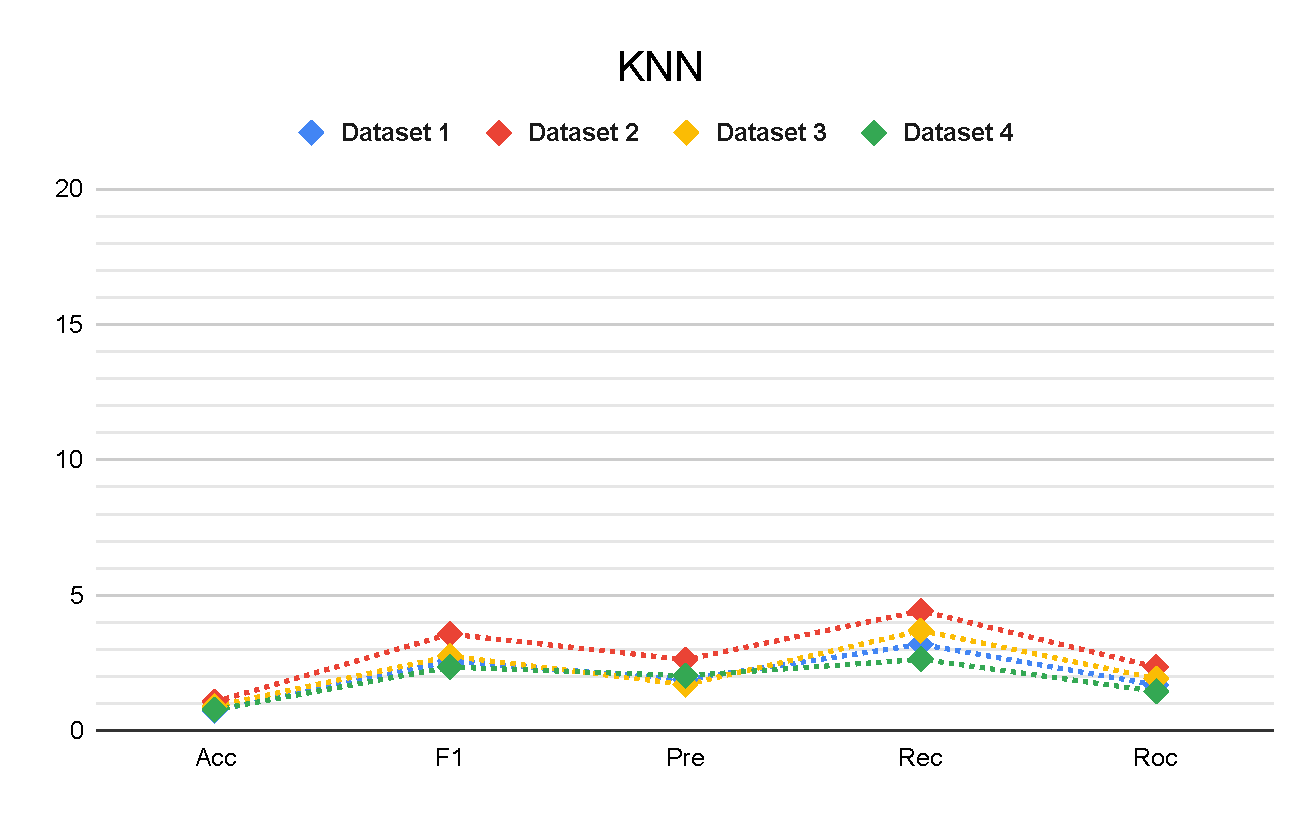
\includegraphics[width=0.9\columnwidth]{media/results/delta_KNN.pdf}
    \caption{Average Error for KNN model} \label{fig:perfromance_delta_knn}
\end{figure}

\begin{figure}[btp]
    \centering
    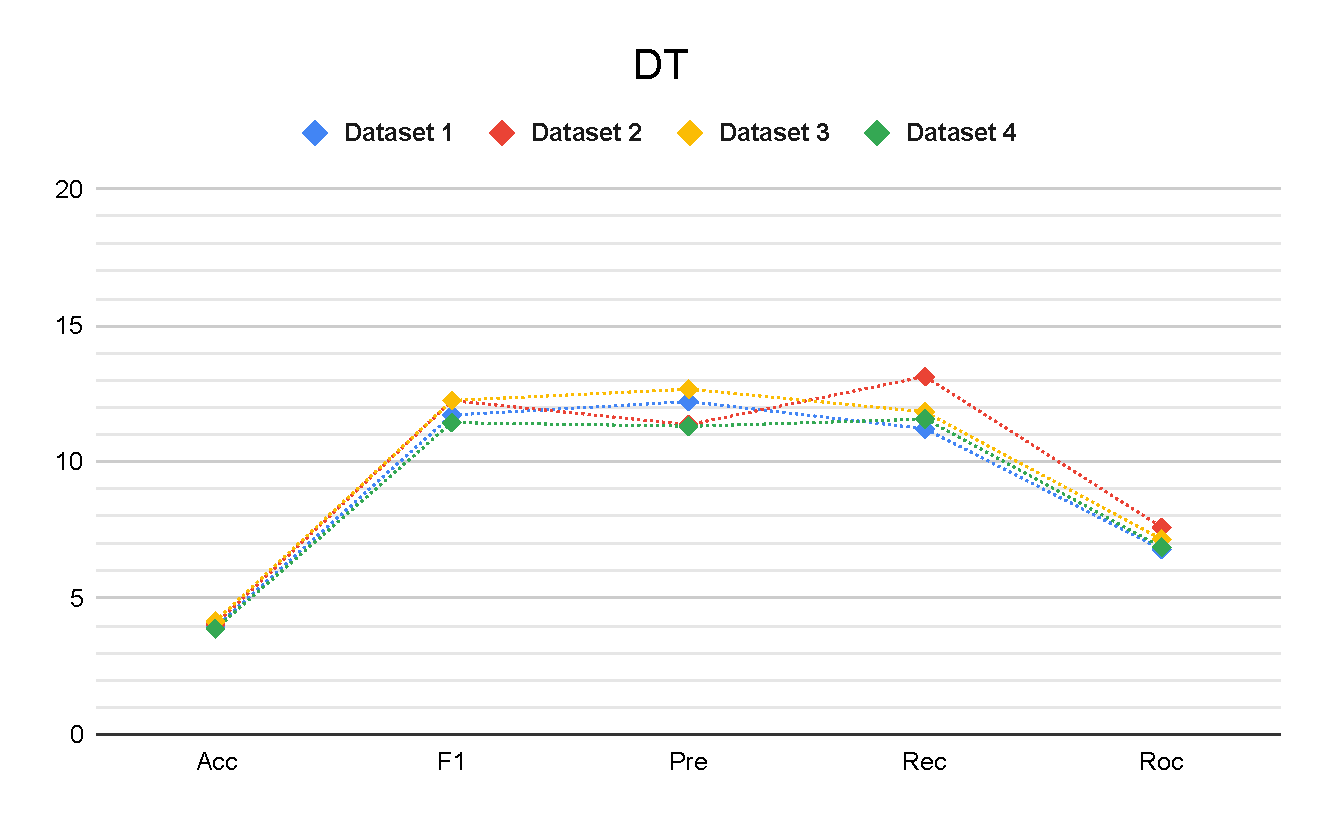
\includegraphics[width=0.9\columnwidth]{media/results/delta_DT.pdf}
    \caption{Average Error for DT model} \label{fig:perfromance_delta_dt}
\end{figure}

\begin{figure}[btp]
    \centering
    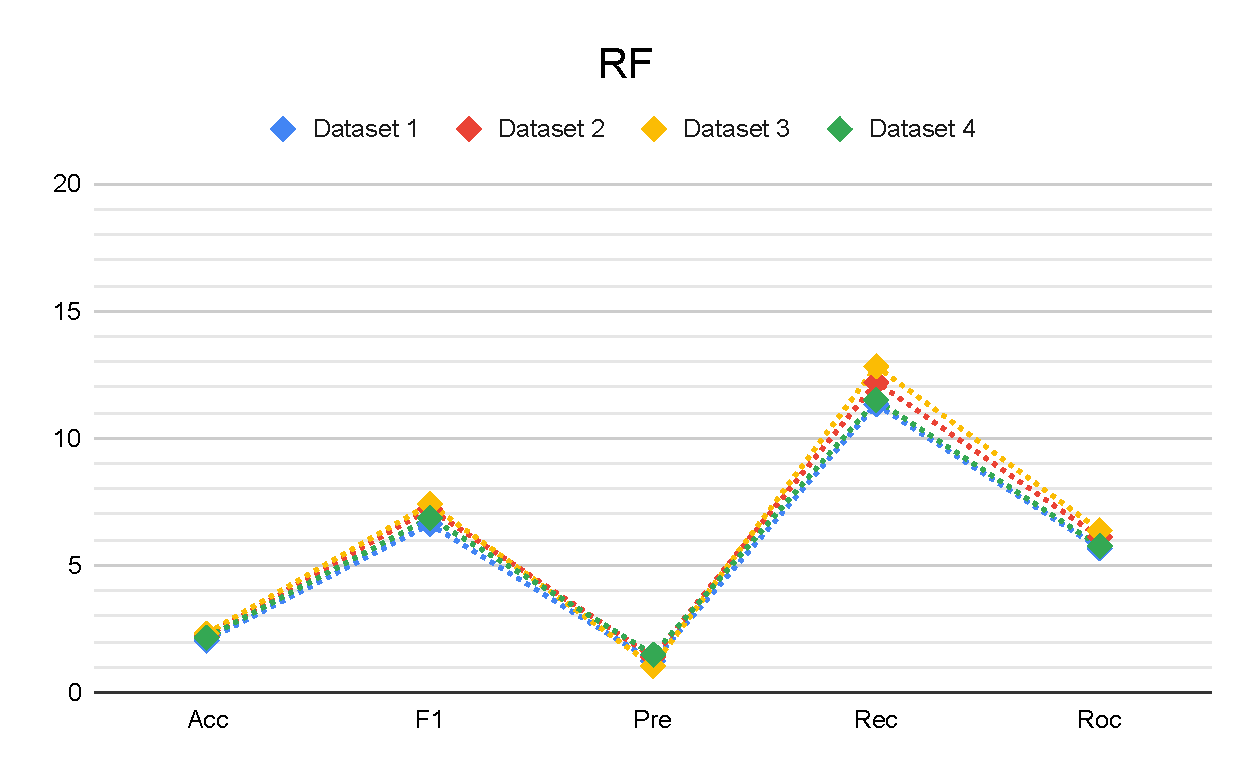
\includegraphics[width=0.9\columnwidth]{media/results/delta_RF.pdf}
    \caption{Average Error for RF model} \label{fig:perfromance_delta_rf}
\end{figure}

\begin{figure}[btp]
    \centering
    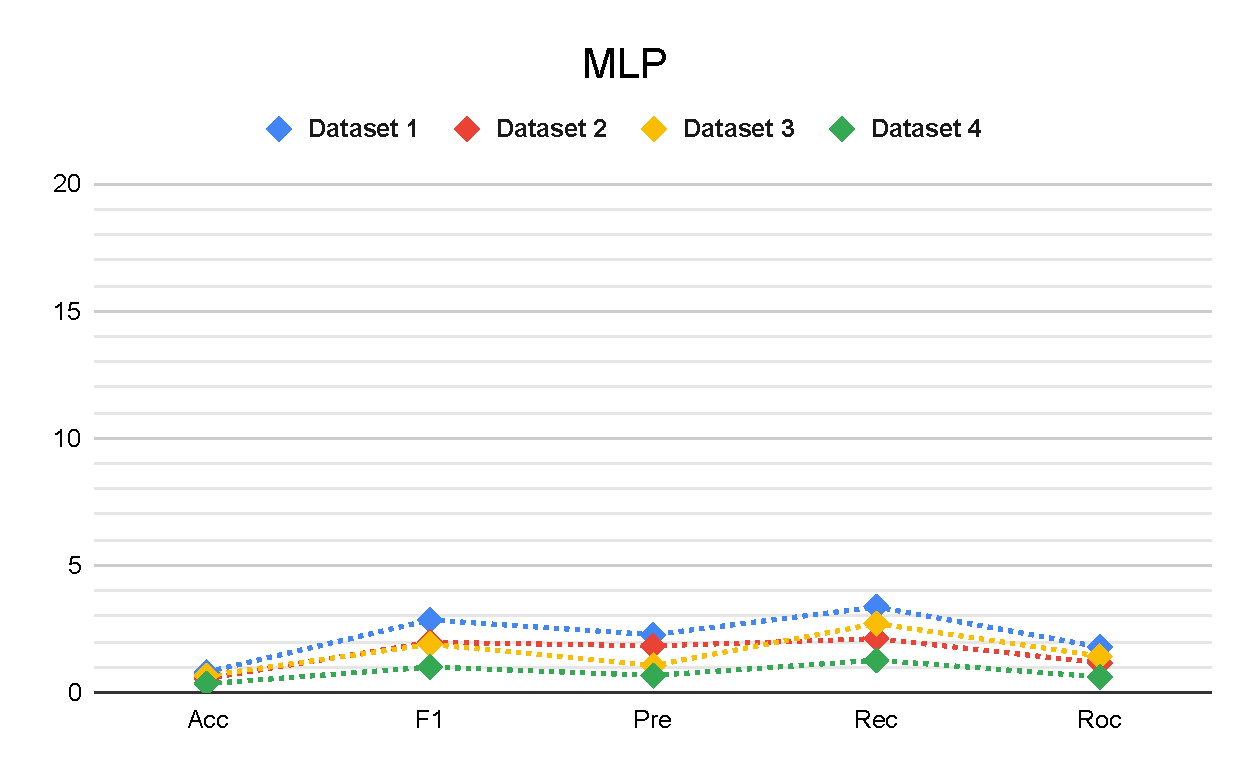
\includegraphics[width=0.9\columnwidth]{media/results/delta_MLP.pdf}
    \caption{Average Error for MLP model} \label{fig:perfromance_delta_mlp}
\end{figure}

\begin{figure}[!tb]
    \centering
    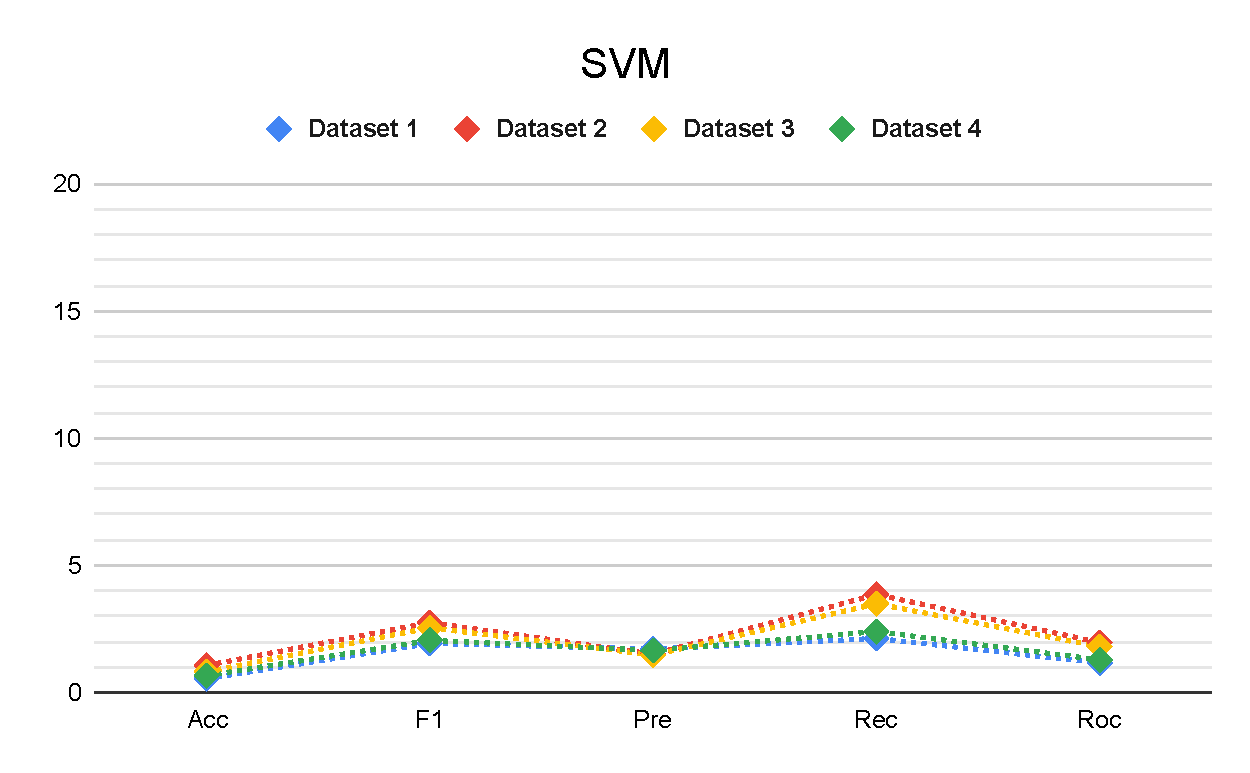
\includegraphics[width=0.9\columnwidth]{media/results/delta_SVM.pdf}
    \caption{Average Error for SVM model} \label{fig:perfromance_delta_svm}
\end{figure}

\section{Conclusion and Future work} \label{sec:conclusion_and_future_work}
In this paper, we present a novel system. The system provides the end user ability to train the best-suited model for the problem. With the current COVID-19 pandemic, this system can be employed by healthcare professionals for the detection of anomalies such as arrhythmia in patients. The system is tested with the ECG MIT-BIH arrhythmia database. The models trained and selected by the system showed good classification performance, these models also performed satisfactorily against training datasets of other models suggesting good general classification performance.

Future work will involve the use of other freely available datasets to test the general classification performance of the system as well as testing the current system in a real-time environment. Also modifying the system to work with non-labeled databases by employing unsupervised learning methods.


% Numbered list
% Use the style of numbering in square brackets.
% If nothing is used, default style will be taken.
%\begin{enumerate}[a)]
%\item 
%\item 
%\item 
%\end{enumerate}  

% Unnumbered list
%\begin{itemize}
%\item 
%\item 
%\item 
%\end{itemize}  

% Description list
%\begin{description}
%\item[]
%\item[] 
%\item[] 
%\end{description}  

% Figure
% \begin{figure}[<options>]
% 	\centering
% 		\includegraphics[<options>]{}
% 	  \caption{}\label{fig1}
% \end{figure}


% \begin{table}[<options>]
% \caption{}\label{tbl1}
% \begin{tabular*}{\tblwidth}{@{}LL@{}}
% \toprule
%   &  \\ % Table header row
% \midrule
%  & \\
%  & \\
%  & \\
%  & \\
% \bottomrule
% \end{tabular*}
% \end{table}

% Uncomment and use as the case may be
%\begin{theorem} 
%\end{theorem}

% Uncomment and use as the case may be
%\begin{lemma} 
%\end{lemma}

%% The Appendices part is started with the command \appendix;
%% appendix sections are then done as normal sections
%% \appendix

% \section{}\label{}

\nocite{*}

% To print the credit authorship contribution details
\printcredits

%% Loading bibliography style file
%\bibliographystyle{model1-num-names}
\bibliographystyle{cas-model2-names}

% Loading bibliography database
\bibliography{cas-refs.bib}

% Biography
\bio{}
% Here goes the biography details.
\endbio

% \bio{pic1}
% Here goes the biography details.
\endbio

\end{document}

